\documentclass{beamer}
\usepackage[utf8x]{inputenc}
\usepackage[ngerman]{babel}
\usepackage{amsmath}
\usepackage{amsfonts}
\usepackage{amssymb}
\usepackage{graphicx}
\usepackage{subfigure}
\author{Johannes Hackel und Falco Prescher}
\title{Testgetriebene Entwicklung}

\usetheme{Ilmenau}
\useoutertheme{split}
\usecolortheme{rose}

\begin{document}

\begin{frame}
\titlepage
\end{frame}

\begin{frame}
\frametitle{Gliederung}
\tableofcontents
\end{frame}

\section{Allgemeines zur testgetriebenen Entwicklung}
\begin{frame}
\frametitle{Definition}
\begin{itemize}
\item Entwicklung von Tests bevor den eigentlichen Komponenten
\item Die Tests definieren das Verhalten
\item Grey-Box-Tests
\end{itemize}
\end{frame}

\begin{frame}
\frametitle{Herkunft}
\begin{itemize}
\item Methode des Extreme Programming (Flexibles Vorgehensmodell)
\item Annäherung an die Anforderungen durch rekursive Zyklen
\item von Kent Beck, Ward Cunningham, Ron Jeffries während Projekt bei Chrysler (1995-2000)
\end{itemize}
\end{frame}

\begin{frame}
\frametitle{Zweck}
\begin{itemize}
\item Qualitätssicherung
\item evolutionäres Design
\item Definition der Schnittstellen $\rightarrow$ modulares Softwaredesign
\end{itemize}
\end{frame}

\begin{frame}
\frametitle{Prinzipien}
\begin{center}
Red $\rightarrow$ Green $\rightarrow$ Refactor
\end{center}
\begin{itemize}
\item Verbesserung des Designs
\item nur neuer Code wenn Test fehlschlägt
\item alle davon abhängige Tests müssen durchgeführt werden
\end{itemize}
\end{frame}

\section{Vorgehensweise der testgetriebenen Entwicklung}
\begin{frame}
\frametitle{Vorgehensweise der testgetriebenen Entwicklung}
\end{frame}

\begin{frame}
\frametitle{Unit Tests}
\end{frame}

\begin{frame}
\frametitle{Testentwurf}
\end{frame}

\begin{frame}
\frametitle{Entwicklungszyklus}
\end{frame}

\section{Das Inversion Of Control im Zusammenhang mit Mocks}
\begin{frame}
\frametitle{Mocks}
\begin{itemize}
\item Mocking - engl. für Vortäuschen
\item Erstellung eines Versuchsobjektes durch eine vorgetäuschte Implementierung von Schnittstellen oder abstrakten Klassen
\item Erzeugung des Objektes während der Laufzeit durch Mockframeworks
\item Implementierung ohne Geschäftslogik
\item Enthalten Konfigurations- und Testverifizierungsmöglichkeiten für Unit Tests
\item Mockframeworks: Mockito\footnote{http://www.code.google.com/p/mockito/} (Java) und Moq\footnote{http://www.code.google.com/p/moq/} (.NET)
\end{itemize}
\end{frame}

\begin{frame}
\frametitle{Inversion Of Control}
\begin{itemize}
\item kurz IoC - engl. für Steuerungsunkehrung
\item Aufrufen von benutzerspezifische Methoden durch das Verhalten eines Softwareframeworks
\item Dependency Injection (DI) = Spezialform des IoC\\Möglichkeit zur Registrierung Schlüssel-Wertpaaren zu einem Container in einer Startsequenz (Bootstrap)
\item Schlüssel = abstrakte Klasse oder Schnittstelle\\Wert = Methode zur Rückgabe eines Objektes (Bsp. Konstruktoren oder Methoden)
\item Inversion Of Control - Frameworks:
PicoContainer\footnote{http://www.picocontainer.codehaus.org/} (Java) und StructureMap\footnote{http://www.docs.structuremap.net/} (.NET)
\end{itemize}
\end{frame}

\begin{frame}
\frametitle{Inversion Of Control}
\begin{figure}[htbp]
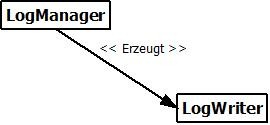
\includegraphics[width=7cm]{logging_closeCoupled.jpg}
\caption{LogManager ist direkt abhängig von einer konkreten Implementierung von LogWriter}
\end{figure}
\end{frame}

\begin{frame}
\frametitle{Inversion Of Control}
\begin{figure}[htbp]
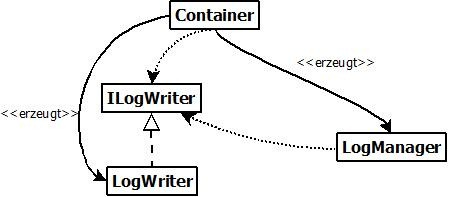
\includegraphics[width=9cm]{logging_looseCoupled.jpg}
\caption{Der Container erzeugt Instanzen und Injiziert Abhängigkeiten}
\end{figure}
\end{frame}

\begin{frame}
\frametitle{Kombination von Inversion Of Control mit Mocks}
\begin{itemize}
\item IoC - Ermöglichen des Benutzens von Mocks zur Testzeit und Produktivcode zur Produktivzeit
\item Mocks - Dadurch lose Kopplung von Programmkomponenten und Testen als einzelnes\\
\item Ohne Inversion Of Control keine Mocks zum Testen nutzbar
\item Ohne Mocks keine testgetriebene Entwicklung für große Programme möglich
\end{itemize}
\end{frame}

\section{Testgetriebene Entwicklung in der Praxis}
\begin{frame}
\frametitle{siehe Beispiel}
\end{frame}

\begin{appendix}
\begin{frame}
\frametitle{Quellen}
\begin{itemize}
\item http://www.codefest.at/post/2009/11/27/Design-Patterns-Teil-1-e28093-Inversion-of-Control-Dependency-Injection.aspx
\item http://www.code.google.com/p/mockito/
\item http://www.code.google.com/p/moq/
\item http://www.webuser.hs-furtwangen.de/kaspar/seminar0607/TestDrivenDevelopement.pdf
\item http://junit.sourceforge.net/javadoc/overview-summary.html
\item OSHEROVE, Roy: the art of UNIT TESTING - with Examples in .NET. Manning Publications Co., 2009
\end{itemize}
\end{frame}
\end{appendix}

\end{document}